\begin{frame}{Background: Max Entropy RL}
\textbf{Conventional RL Objective --- Expected Reward}
\[
\sum_{t} \mathbb{E}_{(\mathbf{s}_t, \mathbf{a}_t) \sim \rho_\pi}\!\left[ r(\mathbf{s}_t, \mathbf{a}_t) \right]
\]

\textbf{Maximum Entropy RL Objective --- Expected Reward $+$ Entropy of the Policy}
\[
\sum_{t} \mathbb{E}_{(\mathbf{s}_t, \mathbf{a}_t) \sim \rho_\pi}\!\left[ r(\mathbf{s}_t, \mathbf{a}_t) + \alpha\, \textcolor{red}{\mathcal{H}(\pi(\,\cdot \mid \mathbf{s}_t))} \right]
\]
\vspace{0.3em}
\begin{itemize}
    \item In words: \emph{``collect reward, \textbf{and} stay as undecided as you can afford to''}
    \item $\alpha$ (the \textbf{temperature}) sets the exchange rate: how much reward is one unit of undecidedness worth?
    \item[$\Rightarrow$] Next two slides: what \emph{is} $\mathcal{H}$, and why does adding it make everything ``soft''?
\end{itemize}
\end{frame}

\begin{frame}{What Is Entropy? (and why the minus sign)}
\small
\textbf{Step 1 --- how surprising is a single outcome?} Define the \emph{surprise} of seeing $x$ as $-\log P(x)$:
\begin{itemize}
    \item $P(x)=1$ (certain) $\Rightarrow -\log 1 = 0$: no surprise at all
    \item $P(x)$ tiny (rare) $\Rightarrow -\log P(x)$ large: very surprising
    \item \textbf{Why a log?} For independent events $P(x,y)=P(x)P(y)$, and $-\log P(x,y) = -\log P(x) - \log P(y)$. Surprises should \emph{add up}, and $\log$ is what turns multiplying into adding
    \item \textbf{Why the minus?} Probabilities are at most $1$, so $\log P(x)$ is negative. The minus just makes surprise a positive number
\end{itemize}
\vspace{0.1em}
\textbf{Step 2 --- entropy is the \emph{average} surprise:}
\hfill
$\displaystyle \mathcal{H}(P) = \mathbb{E}_{x \sim P}\!\big[\, \underbrace{-\log P(x)}_{\text{surprise of }x} \,\big]$
\hfill\mbox{}
\vspace{0.4em}
\begin{center}
\renewcommand{\arraystretch}{1.05}
\scriptsize
\begin{tabular}{@{}lll@{}}
\hline
\textbf{Distribution} & \textbf{Entropy} & \textbf{Reading} \\
\hline
always the same outcome              & $0$                              & fully predictable \\
fair coin                            & $\log 2 \approx 0.69$            & one bit of doubt \\
uniform over $n$ outcomes            & $\log n$ (the largest possible)  & maximally undecided \\
Gaussian $\mathcal{N}(\mu,\sigma^2)$ & $\tfrac12\log(2\pi e \sigma^2)$  & grows with the spread $\sigma$ \\
\hline
\end{tabular}
\end{center}
\end{frame}

\begin{frame}{The Entropy Bonus, One Action at a Time}
\footnotesize
\begin{itemize}
    \item $\mathcal{H}$ is an \emph{average} over actions --- but the agent only ever has the \emph{one} action it sampled. Just unfold the definition:
\end{itemize}
\vspace{-0.3em}
\[
\alpha\,\mathcal{H}(\pi(\,\cdot\mid \mathbf{s}_t)) \;=\; \mathbb{E}_{\mathbf{a}_t \sim \pi}\!\big[\, \textcolor{red}{-\alpha \log \pi(\mathbf{a}_t \mid \mathbf{s}_t)} \,\big]
\]
\begin{itemize}
    \item So per sampled action the bonus is $\textcolor{red}{-\alpha\log\pi(\mathbf{a}_t\mid\mathbf{s}_t)}$: \textbf{the agent is paid extra for taking an action it thought was unlikely.} \emph{This one term is the only thing SAC adds} --- it appears in every equation for the rest of the lecture
    \vspace{0.3em}
    \item Why this fixes DDPG's three problems:
    \begin{itemize}
        \item \textbf{Exploration.} Staying spread out is now \emph{paid for by the objective}, and how much to spread is learned per state --- not a noise schedule you hand-tune
        \item \textbf{Multimodality.} Two equally good actions? Collapsing onto one costs entropy, so the actor keeps both
        \item \textbf{Robustness.} More than one way to act means an alternative survives when the environment shifts
    \end{itemize}
    \vspace{0.3em}
    \item \textbf{Sanity check:} set $\alpha \to 0$ and the bonus vanishes --- what is left is exactly the ordinary RL objective from Day 1. MaxEnt RL is a \emph{strict generalisation}
\end{itemize}
\end{frame}

\begin{frame}{Max Entropy RL}
\begin{itemize}
    \item MaxEnt RL agent can capture different modes of optimality to improve robustness against environmental changes
\end{itemize}
\begin{columns}[c]
\begin{column}{0.5\textwidth}
\centering
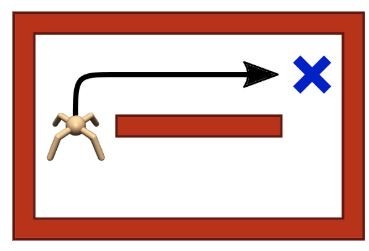
\includegraphics[width=0.9\linewidth,height=0.32\textheight,keepaspectratio]{images/soft-actor-critic/figures/maxent-maze-left.jpg}\\
\vspace{0.2em}
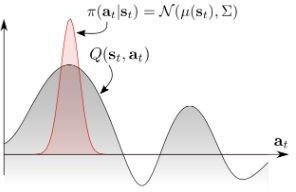
\includegraphics[width=0.9\linewidth,height=0.32\textheight,keepaspectratio]{images/soft-actor-critic/figures/maxent-gauss-left.jpg}
\end{column}
\begin{column}{0.5\textwidth}
\centering
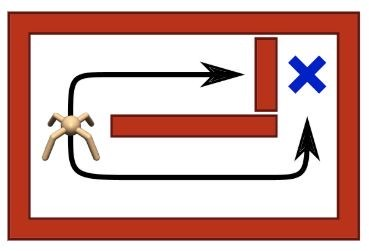
\includegraphics[width=0.9\linewidth,height=0.32\textheight,keepaspectratio]{images/soft-actor-critic/figures/maxent-maze-right.jpg}\\
\vspace{0.2em}
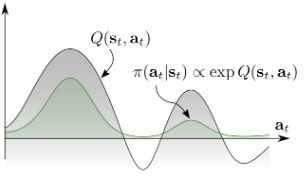
\includegraphics[width=0.9\linewidth,height=0.32\textheight,keepaspectratio]{images/soft-actor-critic/figures/maxent-gauss-right.jpg}
\end{column}
\end{columns}
\begin{flushright}
    \tiny\url{https://bair.berkeley.edu/blog/2017/10/06/soft-q-learning/}
\end{flushright}
\end{frame}

% ---------------------------------------------------------------------------
% The "what does soft mean" trio. Replaces the old KL-to-Boltzmann derivation
% slide (Day 6 review): students have not met partition functions or
% unnormalised densities, and that derivation buried the one idea that
% actually matters -- soft = smooth max. Same conclusion, reached by
% arithmetic instead.
% ---------------------------------------------------------------------------
\begin{frame}{So What Does ``Soft'' Actually Mean?}
\small
\begin{itemize}
    \item $\max_a Q(s,a)$ reports the top score and \emph{throws away everything else}
    \vspace{0.4em}
    \item \textbf{Soft max} $=$ replace it with a smooth version. We \emph{define}:
\end{itemize}
\vspace{-0.2em}
\[
\operatorname{soft\,max}_a Q(s,a) \;=\; \alpha \log \sum_a \exp\!\Big(\tfrac{1}{\alpha}Q(s,a)\Big)
\]
\vspace{-0.2em}
\begin{itemize}
    \item[] {\footnotesize \emph{Reminder:} $\exp(x)$ is just another way of writing $e^x$.}
    \vspace{0.5em}
    \item \textbf{Near-ties get a \emph{bonus}} --- having a good backup plan is worth something
    \vspace{0.2em}
    \item \textbf{A clear winner gets essentially nothing:} it reduces to the plain max
    \vspace{0.2em}
    \item \textbf{It is smooth and differentiable}, unlike $\max$, which jumps the instant the ranking flips
    \vspace{0.5em}
    \item \textcolor{red}{\textbf{The temperature $\alpha$ is the dial:}} $\alpha \to 0$ recovers the hard $\max$ exactly (the largest term swamps the sum); large $\alpha$ washes the differences out and just averages
    \vspace{0.2em}
    \item[] {\footnotesize For continuous actions the sum becomes $\int_{\mathcal{A}}\!\cdots\,d\mathbf{a}$ --- nothing else changes.}
\end{itemize}
\end{frame}

\begin{frame}{Soft Max: Do the Arithmetic}
\small
Two actions, temperature $\alpha = 1$, so $\operatorname{soft\,max} = \log\big(e^{Q_1} + e^{Q_2}\big)$:
\vspace{0.4em}
\begin{center}
\renewcommand{\arraystretch}{1.35}
\small
\begin{tabular}{cccc}
\hline
$Q$ values & hard $\max$ & soft max & the gap \\
\hline
$10,\; 0$    & $10$ & $10.00005$ & $0.00005$ \\
$10,\; 8$    & $10$ & $10.13$    & $0.13$ \\
$10,\; 9.5$  & $10$ & $10.47$    & $0.47$ \\
$10,\; 10$   & $10$ & $10.69$    & $0.69$ \\
\hline
\end{tabular}
\end{center}
\vspace{0.5em}
\begin{itemize}
    \item \textbf{Yes, the soft max is \emph{bigger} than the max --- always.} You are adding a positive quantity to the winner's score, and the closer the runner-up, the bigger it gets. \textbf{That gap \emph{is} the entropy bonus}
    \vspace{0.3em}
    \item Bottom row: the gap is $\log 2 = 0.69$, exactly the entropy of a fair coin --- the payment for genuinely having two options. A runner-up $10$ points behind buys you nothing
    \vspace{0.3em}
    \item \textcolor{red}{\textbf{The dial, concretely.}} On that perfect tie the soft max is exactly $\max + \alpha\log 2$:
    \begin{itemize}
        \item $\alpha = 0 \Rightarrow 10.00$ \quad(the hard max)\qquad $\alpha = 1 \Rightarrow 10.69$ \qquad $\alpha = 2 \Rightarrow 11.39$
    \end{itemize}
\end{itemize}
\end{frame}

\begin{frame}{Why the Soft Max \emph{Is} the Entropy Bonus}
\small
\begin{itemize}
    \item The hard $\max$ asks \emph{which single action is best?} The soft max asks a different question: \emph{which \textbf{distribution} over actions is best, if I am paid $\alpha$ per unit of entropy?}
\end{itemize}
\vspace{-0.2em}
\[
\resizebox{\linewidth}{!}{$\displaystyle
\underbrace{\alpha\log\sum_a \exp\!\big(\tfrac1\alpha Q(s,a)\big)}_{\text{soft max}}
\;=\;
\max_{\pi}\;\Big\{\, \underbrace{\mathbb{E}_{a\sim\pi}[\,Q(s,a)\,]}_{\text{expected value}} \;+\; \underbrace{\alpha\,\mathcal{H}(\pi(\cdot\mid s))}_{\text{entropy bonus}} \,\Big\}
\qquad\text{achieved by}\qquad
\textcolor{red}{\pi(a\mid s) \;\propto\; \exp\!\Big(\tfrac{1}{\alpha}Q(s,a)\Big)}
$}
\]
\begin{itemize}
    \item \textbf{You have met this distribution before.} ``$\propto$'' just means \emph{proportional to} --- written out in full, $\pi(a\mid s)=\dfrac{\exp(Q(s,a)/\alpha)}{\sum_{a'}\exp(Q(s,a')/\alpha)}$, which is the \textbf{softmax} from classification with $Q$-values as the scores and $\alpha$ as the temperature. The bottom line is the normaliser that makes it sum to $1$; the log-sum-exp is that same normaliser read as a value
    \begin{itemize}
        \item $\alpha \to 0$: softmax $\to$ one-hot $\;\Rightarrow\;$ the greedy deterministic policy of Day 2
        \item $\alpha$ large: softmax $\to$ uniform $\;\Rightarrow\;$ random flailing
    \end{itemize}
    \item[$\Rightarrow$] \textbf{One idea wearing three hats:} the soft max (a \emph{value}), the softmax policy (a \emph{distribution}) and ``reward $+\,\alpha\mathcal{H}$'' (an \emph{objective}) are the same statement
\end{itemize}
\end{frame}

\begin{frame}{The ``Soft'' Dictionary}
\small
\begin{center}
\renewcommand{\arraystretch}{1.7}
\begin{tabular}{p{0.10\textwidth} p{0.34\textwidth} p{0.46\textwidth}}
\hline
& \textbf{Hard (Days 1--5)} & \textbf{Soft (today)} \\
\hline
value & $V(s) = \max_a Q(s,a)$
      & $V_{\text{soft}}(s) = \alpha\log\sum_a \exp\!\big(\tfrac1\alpha Q(s,a)\big)$ \\
policy & greedy: $\pi(s) = \arg\max_a Q(s,a)$
      & softmax: $\pi(a\mid s) \propto \exp\!\big(\tfrac1\alpha Q(s,a)\big)$ \\
TD target & $Q \leftarrow r + \gamma \,\textcolor{red}{\max_{a'}}\, Q(s',a')$
      & $Q \leftarrow r + \gamma \,\textcolor{red}{\operatorname{soft\,max}_{a'}}\, Q(s',a')$ \\
objective & $\sum_t \mathbb{E}\big[\,r_t\,\big]$
      & $\sum_t \mathbb{E}\big[\,r_t + \alpha\mathcal{H}(\pi(\cdot\mid \mathbf{s}_t))\,\big]$ \\
\hline
\end{tabular}
\end{center}
\vspace{0.1em}
{\footnotesize
\begin{itemize}
    \item Every row is the \emph{same single substitution}. Nothing else from Days 1--5 changes: replay buffer, target networks, TD updates and clipped double-$Q$ all carry over untouched
    \item Set $\alpha \to 0$ and every right-hand entry collapses back to the left --- ``soft'' costs you nothing, it only adds a dial
\end{itemize}
\vspace{0.3em}
\textcolor{red}{\textbf{The TD-target row is the one that changes your code.}} Every value method since Day 2 has bootstrapped with $\max_{a'}Q(s',a')$ inside the TD target. \textbf{In MaxEnt RL that $\max$ is replaced by the soft max --- nothing else about TD learning changes.} And once you have an actor to sample from, the soft max is computed as $\mathbb{E}_{a'\sim\pi}[\,Q(s',a') - \alpha\log\pi(a'\mid s')\,]$, so no exponential ever appears in the code.}
\end{frame}
